\documentclass{report}
\usepackage[utf8]{inputenc}
\usepackage[spanish]{babel}
\usepackage[margin=2cm]{geometry}
\usepackage{graphicx}
\usepackage{float}
\usepackage{titlesec}
\usepackage{caption}
\usepackage{listings}
\usepackage{xcolor}
\usepackage{array}
\usepackage{booktabs}
\usepackage{tabularx}
\usepackage{multirow}
\usepackage{amsmath}
\usepackage{hyperref}
\usepackage{ragged2e} 
\usepackage{lipsum}

\definecolor{codegreen}{rgb}{0,0.6,0}
\definecolor{codegray}{rgb}{0.5,0.5,0.5}
\definecolor{codepurple}{rgb}{0.58,0,0.82}
\definecolor{backcolor}{rgb}{0.95,0.95,0.95}

\lstset{
    basicstyle=\ttfamily,
    inputencoding=utf8,
    extendedchars=true,
    literate=%
    {á}{{\'a}}1
    {é}{{\'e}}1
    {í}{{\'i}}1
    {ó}{{\'o}}1
    {ú}{{\'u}}1
    {ñ}{{\~n}}1
    {Á}{{\'A}}1
    {É}{{\'E}}1
    {Í}{{\'I}}1
    {Ó}{{\'O}}1
    {Ú}{{\'U}}1
    {Ñ}{{\~N}}1
}

\lstdefinestyle{mystyle}{
    backgroundcolor=\color{backcolor},
    commentstyle=\color{codegreen},
    keywordstyle=\color{red},
    numberstyle=\tiny\color{codegray},
    stringstyle=\color{codepurple},
    basicstyle=\ttfamily\footnotesize,
    breakatwhitespace=false,
    breaklines=true,
    captionpos=b,
    keepspaces=true,
    numbers=left,
    showspaces=false,
    showstringspaces=false,
    showtabs=false,
    tabsize=2  
}

\titleformat{\section}
{\huge\bfseries}{\thesection.}{1em}{}
\titleformat{\subsection}
{\large\bfseries}{\thesubsection}{1em}{}

\renewcommand\thesection{\arabic{section}}

\title{\Huge{\textbf{Modelo de Procesos y Modelo de Datos}}\\
\Large{\textbf{Ingeniería de Software Para Sistemas Intelgentes}}}
\author{Diego Castillo Reyes\\Marthon Leobardo Yañez Martinez\\Aldo Escamilla Resendiz}

\graphicspath{{imagenes/}}

\begin{document}
\maketitle
\section{Modelo de Procesos}
\subsection*{Diagrama de Secuencia}
A continuación de mostrará el diagrama de secuencia donde se
muestra el proceso del sistema:
\begin{figure}[H]
    \centering
    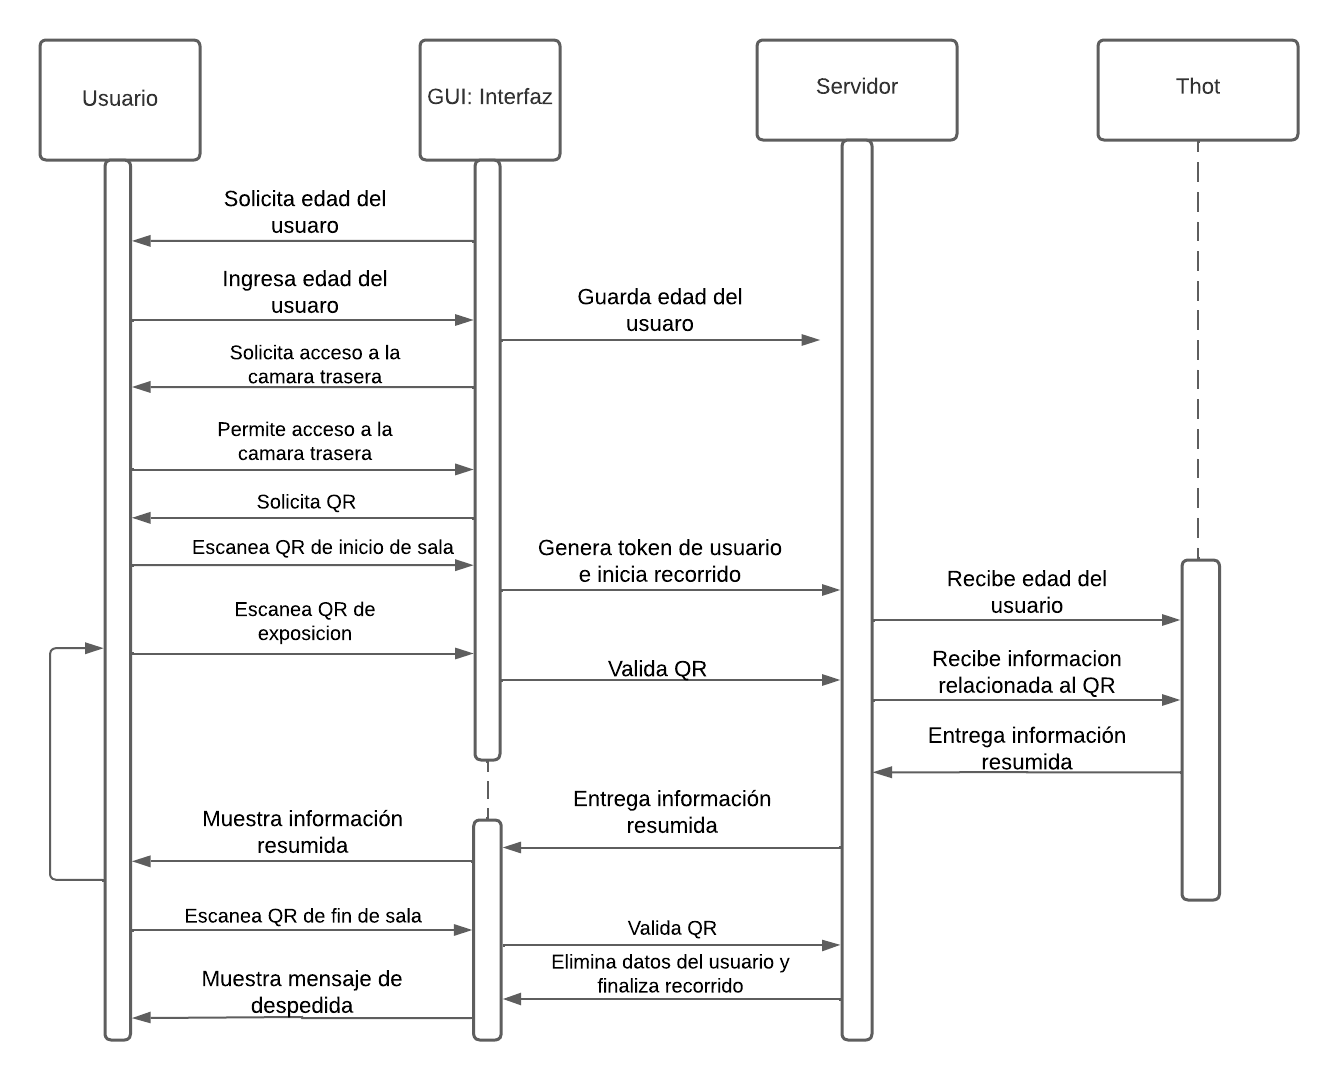
\includegraphics[width=0.8\textwidth]{Diagrama de secuencia.png}
    \caption{Diagrama de Secuencia}
\end{figure}
\subsection*{Descripción de Procesos}
\begin{itemize}
    \item Inicio del recorrido: El usuario ingresa su edad, el sistema guarda el dato y le permite escanear el QR de inicio de sala.
    \item Recorrido interactivo: A medida que el usuario escanea los QR de la exposición, el sistema Thot genera resúmenes personalizados que se muestran en la interfaz del usuario.
    \item Finalización del recorrido: El usuario escanea el QR de salida, el servidor valida el escaneo y elimina los datos del usuario. Finalmente, el sistema muestra un mensaje de despedida al usuario.
\end{itemize}

\newpage

\section{Modelo de Datos}
\subsection*{Diagrama de Entidad-Relación}

A continuación se muestra el diagrama de entidad-relación del sistema:

\begin{figure}[H]
    \centering
    \includegraphics[width=0.8\textwidth]{Entidad-Relación Museo.png}
    \caption{Diagrama de Entidad-Relación}
\end{figure}

\subsection*{Descripción de Entidades y Relaciones}

\begin{enumerate}
    \item \textbf{Entidad Visitante}:
    \begin{itemize}
        \item Representa a los usuarios que interactúan con el sistema.
        \item \textbf{Atributos}:
        \begin{itemize}
            \item \texttt{ID\_visitante}: Identificador único.
            \item \texttt{Nombre}: Nombre del visitante.
            \item \texttt{Edad}: Edad del visitante.
            \item \texttt{Puntuación\_trivia}: Puntuación acumulada en trivias.
        \end{itemize}
        \item \textbf{Relación con Actividad (1:N)}: Un visitante puede realizar múltiples actividades, pero cada actividad está relacionada con un solo visitante.
    \end{itemize}

    \item \textbf{Entidad Actividad}:
    \begin{itemize}
        \item Representa una acción realizada por el visitante, como participar en una trivia o explorar un resumen.
        \item \textbf{Atributos}:
        \begin{itemize}
            \item \texttt{Tipo}: Tipo de actividad (e.g., trivia, exploración).
            \item \texttt{Fecha}: Fecha de realización.
            \item \texttt{Puntuación\_trivia}: Puntuación obtenida en una trivia específica.
            \item \texttt{ID\_visitante}: Relación con el visitante que realizó la actividad.
        \end{itemize}
        \item \textbf{Relación con Trivia (1:1)}: Cada actividad está asociada a una sola trivia, representando la interacción directa del visitante con el contenido educativo.
    \end{itemize}

    \item \textbf{Entidad Trivia}:
    \begin{itemize}
        \item Representa una serie de preguntas relacionadas con los objetos históricos, diseñadas para probar los conocimientos del visitante.
        \item \textbf{Atributos}:
        \begin{itemize}
            \item \texttt{ID\_trivia}: Identificador único.
            \item \texttt{Pregunta}: La pregunta de trivia.
            \item \texttt{Respuesta}: Respuesta correcta.
            \item \texttt{Opciones}: Posibles respuestas.
            \item \texttt{Puntuación\_trivia}: Puntuación otorgada por esa trivia.
        \end{itemize}
        \item \textbf{Relación con Objeto Histórico (N:N)}: Las preguntas de trivia están relacionadas con uno o más objetos históricos, y un objeto puede estar vinculado con varias trivias.
    \end{itemize}

    \item \textbf{Entidad Sala}:
    \begin{itemize}
        \item Representa las salas del museo donde se encuentran los objetos históricos.
        \item \textbf{Atributos}:
        \begin{itemize}
            \item \texttt{ID\_sala}: Identificador único.
            \item \texttt{Nombre\_sala}: Nombre de la sala.
        \end{itemize}
        \item \textbf{Relación con Objeto Histórico (1:N)}: Cada sala contiene varios objetos históricos, pero cada objeto pertenece a una única sala.
    \end{itemize}

    \item \textbf{Entidad Objeto Histórico}:
    \begin{itemize}
        \item Representa los objetos expuestos en el museo, sobre los cuales se generan resúmenes y trivias.
        \item \textbf{Atributos}:
        \begin{itemize}
            \item \texttt{ID\_objeto}: Identificador único.
            \item \texttt{Nombre\_objeto}: Nombre del objeto.
            \item \texttt{Descripción}: Descripción del objeto.
            \item \texttt{Información}: Información relevante del objeto que se sintetiza en los resúmenes.
        \end{itemize}
        \item \textbf{Relación con Resumen (N:N)}: Un objeto puede tener varios resúmenes generados por Thot, y cada resumen puede incluir información sobre varios objetos.
    \end{itemize}

    \item \textbf{Entidad Resumen}:
    \begin{itemize}
        \item Representa los resúmenes generados automáticamente por el sistema Thot a partir de los objetos históricos.
        \item \textbf{Atributos}:
        \begin{itemize}
            \item \texttt{ID\_Resumen}: Identificador único.
            \item \texttt{Texto}: Contenido resumido.
            \item \texttt{ID\_objeto}: Relación con el objeto histórico al que pertenece.
        \end{itemize}
    \end{itemize}
\end{enumerate}


\end{document}